\setlength{\headheight}{14pt}
\section{Neural Processing Unit (NPU) and Neural Engines}
\subsection{What is an NPU?}

Neural Processing Unit (NPU) is a processing unit like CPU and a GPU but specialized for 
Artificial Intelligence and Machine Learning Tasks. CPU designed to handle many different 
general purpose tasks and GPU mainly designed to perform graphics and parallel calculation 
when the NPU is mainly designed to perform  mathematical operations used by neural networks 
such as, working with vectors and tensors. NPU is not a unit that replaces the CPU 
and the GPU; instead, they work together and each processor handles the type of work 
it is best suited for (heterogeneous computing). In modern devices such as smart phones , 
laptops and other smart electronic devices , the NPU is usually integrated with CPU and 
GPU inside a single System on Chip (Soc) to perform Artificial Intelligence tasks such as 
face recognition, speech recognition and image enhancement ect. Since Neural Processing 
Units (NPU) are specialized for AI workloads, they can provide high performance with 
relatively lower power consumption than CPUs and GPUs.

\subsection{Architecture and Operation}
\begin{figure}[H]
    \centering
    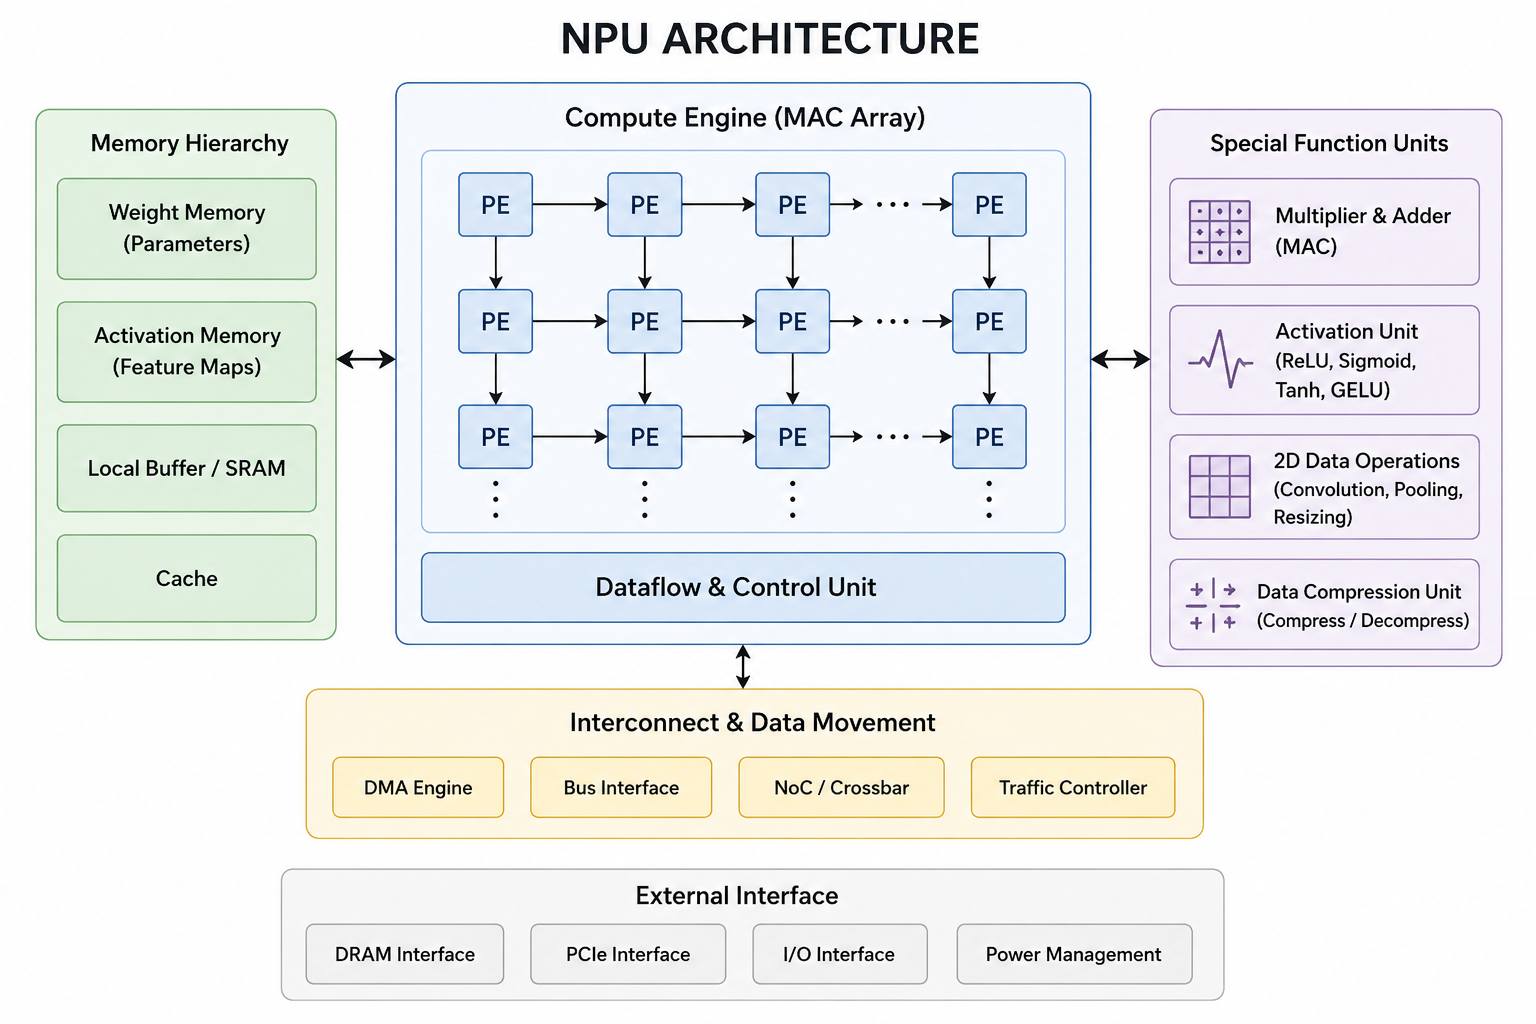
\includegraphics[width=0.85\textwidth]{images/NPU Archi.png}
    \caption{Simplified NPU Architecture}
\end{figure}


The Neural Processing Unit architecture is the internal organization of specialized hardware that is 
designed to perform neural network operations. A neural-network accelerator (NPU) contains a compute 
engine with many Processing Elements (PEs) that perform small calculations such as multiplications and 
accumulation (MAC), which are the fundamentals of neural-network calculations. Research on the Eyeriss 
accelerator demonstrates how parallel processing elements can be organized to efficiently execute 
convolutional neural networks while reducing energy consumption \cite{paper_1}. Similarly, Google’s TPU 
(Tensor Processing Unit) uses a large matrix of MAC units as its main computational engine. 
That shows the high importance of parallel computation in AI accelerators \cite{paper_2}. NPUs require an 
efficient memory hierarchy to store neural-network weights, input data, and intermediate results. 
Also, keeping frequently used data close to the processing unit reduces expensive data movements and 
improves energy efficiency \cite{paper_1}. In addition, the data flow and interconnect mechanism control how data 
moves between the memory and the processing elements. Eyeriss v2, for example, uses a flexible on-chip 
network to adapt data movement to different neural-network workloads \cite{paper_3}. 
Therefore, the NPU architecture mainly combines parallel processing elements, MAC units, local memory, 
data movement networks, and control mechanisms to achieve high performance and 
energy-efficient AI processing [1–3].

\subsection{Applications}
Neural Processing Units are mainly used to improve Artificial Intelligence and Machine Learning tasks. 
One important application of NPUs is Smartphones. Smartphones use NPUs for image enhancements, 
face recognition, speech processing, and other AI-based features with low power consumption \cite{paper_4}. 
NPUs are also useful in computer vision, including real-time image processing, object detection 
and image classification \cite{paper_1}. In IoT and edge devices, they can use sensors and AI data locally 
by reducing latency and dependence on cloud servers \cite{paper_5}. NPUs can support healthcare, robotics, 
autonomous systems and smart environments, where fast AI interfaces are required \cite{paper_5}. As AI models 
become more common on modern edge devices, specialized neural-network accelerators are more 
important for achieving real-time performance within limited power and computing resources \cite{paper_5}.

\subsection{Advantages and Limitations}
NPUs provide high performance and energy efficiency for AI work since they use specialized hardware and 
massive parallel processing for neural-network operations \cite{paper_6}. They can reduce data movement and reuse 
data locally, which helps to lower power consumption and improve processing efficiency \cite{paper_6}. NPUs are 
especially useful for real-time AI applications on mobile and edge devices where performance and battery 
life are important \cite{paper_7}. 
There are some limitations also.  NPU may be less flexible than a CPU or GPU when running different or 
rapidly changing neural-network models \cite{paper_7}, \cite{paper_8}. Because some accelerator designs work best only with 
specific model characteristics, such as particular data patterns or sparsity \cite{paper_8}. In addition, specialized 
hardware can require greater design complexity and become less efficient when the workload does not match 
its architecture \cite{paper_7}. Therefore, NPUs provide excellent AI performance per watt, but this advantage comes 
with trade-offs in flexibility, programmability, and workload compatibility.

\subsection{Future Trends}
In the future NPU development is expected to focus on higher energy efficiency, greater parallelism, and 
improved support for increasingly complex AI models \cite{paper_9}. NPUs are becoming more important in edge AI, 
allowing devices such as smartphones, IoT systems, robots and vehicles to process AI locally with low latency \cite{paper_10}. 
Researchers are exploring quantization, sparsity, model compression and memory-centric architecture to reduce the 
computation and data movement cost \cite{paper_9}, \cite{paper_11}.  
Another emerging direction is on-device learning, which allows AI models to adapt directly to changing environments \cite{paper_12}. 
However, future NPUs face challenges including limited memory, high data movement cost, hardware complexity, model 
compatibility, scalability, and power constraints \cite{paper_9}, \cite{paper_11}.  As a result of that, future NPU research will increasingly 
focus on hardware-software co-design, flexible architectures, efficient memory systems and specialized support for 
emerging AI workloads.
